\documentclass{article}
\usepackage[utf8]{inputenc}
\usepackage{enumitem}
\usepackage{bm}
\usepackage[margin=1.0in]{geometry}

\title{Physics 116B \\ Mathematical Methods in Physics\\ Small Group Tutoring}
\author{Pablo Sevilla}
\date{Week 9 - May 30 2018}

\usepackage{natbib}
\usepackage{graphicx}

\begin{document}
\maketitle

\begin{figure}[h]
\centering

\includegraphics[scale=0.3]{lss}
\end{figure}
\section{Preliminary Questions}
 \begin{itemize}
  \item A line integral is an integral where the function to be integrated is evaluated along a curve. The terms path integral, curve integral, and curvilinear integral are also used. One of the many applications in physics is calculating the work done by a particle in a field travelling along a path C. Contour integral are typically reserved for line integrals in the complex plane. Find the following Contour Integrals:
\begin{figure}[h]
\centering
\begin{subfigure}{\textwidth}
  \centering
  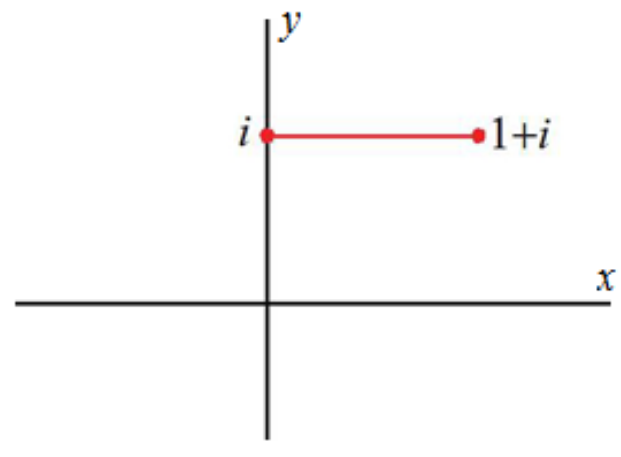
\includegraphics[width=.3\linewidth]{P1}
\end{subfigure}%
\begin{subfigure}{\textwidth}
  \centering
  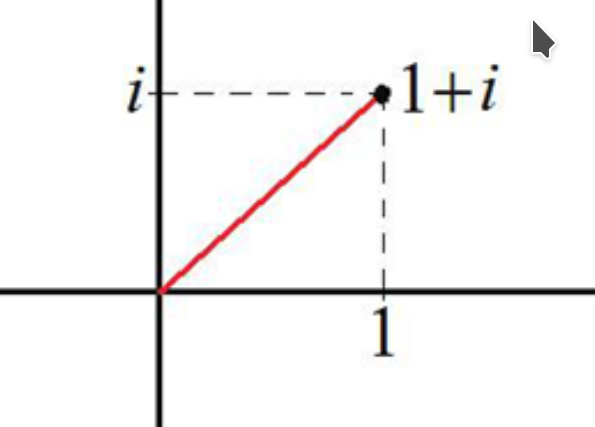
\includegraphics[width=.3\linewidth]{P2}
\end{subfigure}
\end{figure}

\item Cauchy's Theorem states that
\begin{equation}
    \oint_C f(z)dz=0
\end{equation}
along a closed curve $C$. Under what condition does this hold? If this is true, how can you obtain the value of $f(z)$ at a point $z=a$ inside $C$? Refer to the textbook.
\item A Laurent series of a complex function $f(z)$ is a representation of that function as a power series which includes terms of negative degree. It may be used to express complex functions in cases where a Taylor series expansion cannot be applied. They are expressed as:
\begin{equation}
    f(z) = \sum_{n=-\infty}^{\infty} a_n(z-z_0)^n
\end{equation}
When all the negative $n$ terms are zero, what can we say about $f(z)$ at $z=z_o$? And what if one, a few or all these terms are non-zero? This brings us to the Residue Theorem. This is extremely useful when taking a Contour integral of a closed curve $C$ that is analytic except of several isolated singularities $z_0, z_1, z_2,...$, as shown in the figure below. What is the value of the Contour integral in this case?
\begin{figure}[h]
    \centering
    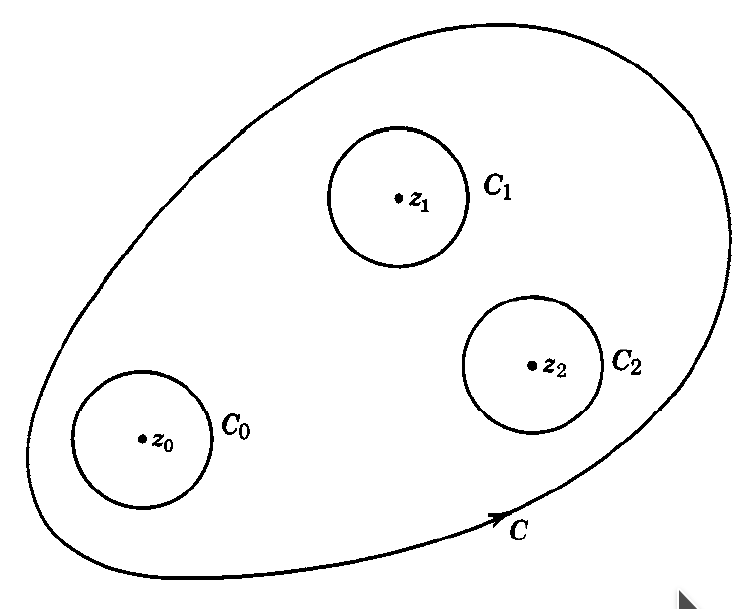
\includegraphics[width=.2\linewidth]{P4}
\end{figure}
 \end{itemize}
  

  \section{Group Problems}
  Work together as a group for the following problems. Once solved, prepare a presentation to explain the problems in an organized manner.
  \subsection{Problem 1}
  Show that by differentiating Cauchy's formula $n$ times, you obtain the following relationship:
  \begin{equation}
      \frac{d^n}{dz^n}\Bigg(f(a)\Bigg)=\frac{d^n}{dz^n}\Bigg(\frac{1}{2\pi i}\oint_C \frac{f(z)}{z-a}dz\Bigg)=\frac{n!}{2\pi i}\oint_C \frac{f(z)}{(z-a)^{n+1}}dz
  \end{equation}
  \subsection{Problem 2}
  Find all the residues of the following complex functions:
  
\begin{enumerate}
    \item $\frac{1}{(1-2z)(5z-4)}$
    \item $\frac{1}{z(1-z)}$
    \item $\frac{z}{1-z^4}$
    \item $\frac{cosz}{1-2sinz}$
    \item $\frac{z}{(z^2+1)^2}$
\end{enumerate}
  \subsection{Problem 3}
  The following integrals are often found in integral tables used in many areas of physics, such as Quantum Mechanics. Evaluate the following integrals by the methods you have recently learned:
  \begin{enumerate}
    \item $\int_{0}^{2\pi}\frac{1}{13+5\sin{\theta}}d\theta$
    \item $\int_{0}^{2\pi}\frac{\sin^2{\theta}}{5+3\cos{\theta}}d\theta$
\end{enumerate}
  
\end{document}
